\documentclass{bmstu}

\bibliography{biblio}

\begin{document}

\makereporttitle
    {Информатика, искусственный интеллект и системы управления} % Название факультета
    {Программное обеспечение ЭВМ и информационные технологии} % Название кафедры
    {лабораторной работе №~1} % Название работы (в дат. падеже)
    {Защита Информации} % Название курса (необязательный аргумент)
    {Энигма} % Тема работы
    {} % Номер варианта (необязательный аргумент)
    {Корниенко~К.~Ю./ИУ7-71Б} % Номер группы/ФИО студента (если авторов несколько, их необходимо разделить запятой)
    {Чиж~И.~С.} % ФИО преподавателя

\maketableofcontents

\chapter*{ВВЕДЕНИЕ}
\addcontentsline{toc}{chapter}{ВВЕДЕНИЕ}

Цель лабораторной работы --- разработать программу шифровальной машины <<Энигма>> \cite{Enigma}.

Задачи лабораторной работы:

\begin{enumerate}[label=---]
    \item провести анализ устройства шифровальной машины <<Энигма>>;
    \item описать алгоритм шифрования <<Энигмы>>;
    \item реализовать описанный алгоритм;
    \item протестировать работу алгоритма на текстовых и бинарных файлах.
\end{enumerate}

\chapter{Аналитический раздел}

\section{Алгоритм шифрования <<RSA>>}

RSA --- криптографический алгоритм с открытым ключом, основывающийся на вычислительной сложности задачи факторизации.

Алгоритм:

\begin{enumerate}
	\item Выбираем два случайных простых числа $p$ и $q$.
	\item Вычисляем их произведение: $N = p \times q$.
	\item Вычисляем функцию Эйлера: $\phi(N) = (p - 1) \times (q - 1)$.
	\item Выбираем число $e$ (обычно простое, но необязательно), которое меньше $\phi(N)$ и является взаимно простым с $\phi(N)$.
	\item Ищем число $d$, обратное числу $e$ по модулю $\phi(N)$:
	\begin{equation*}
		d \times e \equiv 1 ~~ (\textrm{mod} ~~ \phi(N)).
	\end{equation*}

	Найти его можно через расширенный алгоритм Евклида.
\end{enumerate}

\section{Алгоритм хеширования <<MD5>>}

MD5 --- 128-битный алгоритм хеширования, разработанный профессором Рональдом Л. Ривестом из Массачусетского технологического института (Massachusetts Institute of Technology, MIT) в 1991 году.
Предназначен для создания «отпечатков» или дайджестов сообщения произвольной длины и последующей проверки их подлинности.
Широко применялся для проверки целостности информации и хранения хешей паролей, однако признан небезопасным из-за малой длины получаемого хэша и простотой самого алгоритма.

\chapter{Конструкторская часть}

\section{Разработка алгоритма}

На рисунке \ref{fig:algo} представлена схема создания и проверки цифровой подписи.

\begin{figure}[h!]
	\centering
	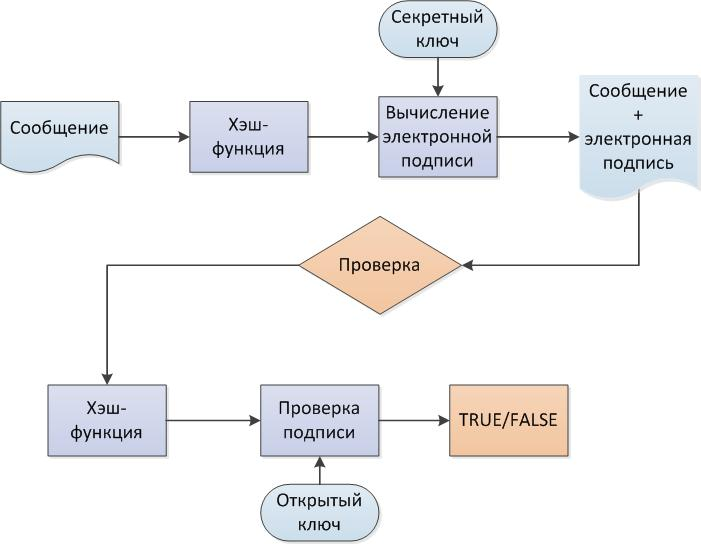
\includegraphics[width=0.85\textwidth]{img/RSA.jpeg}
	\caption{Схема создания и проверки цифровой подписи}
	\label{fig:algo}
\end{figure}
\clearpage

\chapter{Технологическая часть}

\section{Средства реализации}

Для реализации ПО был выбран язык C++ \cite{C++}.
В данном языке есть все требующиеся инструменты для данной лабораторной работы.
В качестве среды разработки была выбрана среда VS code \cite{vscode}.

\section{Реализация алгоритма}

Реализация кодирования LZW.

\begin{lstlisting}
void compressInternal(const std::vector<uint8_t>& inputFile)
{
    initializeDictionary();

    std::vector<uint8_t> currentSubsequence;
    int nextIndex = 0;
    uint8_t nextByte;
    TrieNode* currentNode = rootNode;

    int code = 0xFF + 1;

    while (nextIndex < inputFile.size())
    {
        nextByte = inputFile[nextIndex];
        if (currentNode->children.contains(nextByte))
        {
            currentNode = &currentNode->children[nextByte];
            nextIndex++;
        }
        else
        {
            tempOut->emplace_back(currentNode->code, getBitsToRepresentInteger(code));
            currentNode->children[nextByte].code = code;
            code++;
            currentNode = rootNode;
        }
    }

    if (currentNode != rootNode)
    {
        tempOut->emplace_back(currentNode->code, getBitsToRepresentInteger(code));
    }

    std::cout << "dict size: " << getDictSize() << std::endl;
}
\end{lstlisting}

\section{Тестирование ПО}

В таблице \ref{tbl:functional_test} приведены тесты для алгоритма шифрования LZW. 
Применена методология черного ящика. Тесты пройдены \textit{успешно}.

\begin{table}[ht!]
	\begin{center}
		\captionsetup{justification=raggedright,singlelinecheck=off}
		\caption{\label{tbl:functional_test} Функциональные тесты}
		\begin{tabular}{|c|c|c|}
			\hline
			Входная строка & Размер входной (Байт) & Размер выходной (Байт) \\ 
			\hline
			$aba$          & 3  & 4 \\
			$abaaba$       & 6  & 6 \\
			<<>>           & 0  & 0 \\
            $abaabaabaaba$ & 12 & 8 \\
			\hline
		\end{tabular}
	\end{center}
\end{table}

\chapter*{ЗАКЛЮЧЕНИЕ}
\addcontentsline{toc}{chapter}{ЗАКЛЮЧЕНИЕ}

В данной лабораторной работе:

\begin{enumerate}[label=---]
    \item проведен анализ работы алгоритма сжатия <<LZW>>;
    \item описан алгоритм сжатия;
    \item реализован описанный алгоритм.
\end{enumerate}


\makebibliography

\end{document}